\chapter[~]{Визначення мінімального шляху на графі з ребрами довільної довжини}

\textbf{Мета роботи} --- Навчитися визначати оптимальний шлях (мінімальної довжини) у заданого
графа, а також виконувати синтез графа (визначення ваги всіх ребер та індексів усіх вершин), що має
задану структуру та заданий оптимальний шлях.

\section{ Короткі теоретичні відомості}

Є багато підходів до визначення поняття ``граф''. Наведемо одне з таких визначень. Нехай $V$ ---
довільна множина, $E$ --- деяка сукупність пар вигляду $(v_i , v_j)$, де $v_i , v_j \in V$ (тобто
сукупність пар елементів, що входять до множини $V$), причому в сукупності $E$ можуть зустрічатися
однакові пари. Тоді упорядкована пара $G=(V, E)$, що складається з множини $V$ та сукупності $E$,
називається \emph{графом} із множиною вершин $V$ та множиною ребер $E$.

Іншими словами, \emph{граф} --- це дві множини, що взаємно відповідають одна інший, --- множина вершин
та множина ребер (множина бінарних відношень вершин), кожне (ребро) з яких відповідає парі елементів
(допускаються однакові елементи) з множини вершин.

Графи зручно зображати графічно (малюнком), що спричинило появу їхньої назви. При цьому елементи
множини вершин $V$ зображають крапками на площині, а ребра ($v_i,$ $v_j$) --- відрізками
(прямолінійними або криволінійними), які з'єднують крапки $v_i$ та $v_j$.

Граф називається \emph{скінченним}, якщо множини його вершин та ребер є скінченими (надалі
розглядаються лише такі графи). Множину вершин графа $G$ позначають $V(G)$, а множину ребер ---
$E(G)$. Кількість вершин графа $n(G)=|V(G)|$ (кількість елементів $V(G)$). Кількість ребер графа
$m(G)=|E(G)|$ (кількість елементів $E(G)$). Кількість вершин графа називають його \emph{порядком}.

Якщо елемент $e$ (ребро) сукупності $E$ є парою елементів (вершин) $v$ та $w$: $e = (v, w)$, то
кажуть:

\begin{itemize}
\item вершини $v$ та $w$ суміжні;
\item вершини $v$ та $w$ є кінцями ребра $e$;
\item вершини $v$ та $w$ --- інцидентні ребру $e$;
\item ребро $e$ --- інцидентне вершинам $v$ та $w$.
\end{itemize}

Іншими словами, якщо вершини є кінцями ребра, то вони \emph{інцидентні} цьому ребру, а ребро ---
інцидентне їм. Два ребра називають \emph{суміжними}, якщо обидва вони є інцидентними одній вершині
(тобто мають спільну вершину). Кількість ребер, інцидентних деякій вершині $v$, називається
локальним степенем або просто \emph{степенем вершини} $v$.

Графічне представлення деяких прикладів графів наведено на \ref{f:graph_examples}.

\begin{figure}[!ht]
  \begin{subfigure}{.25\textwidth}
    \centering
    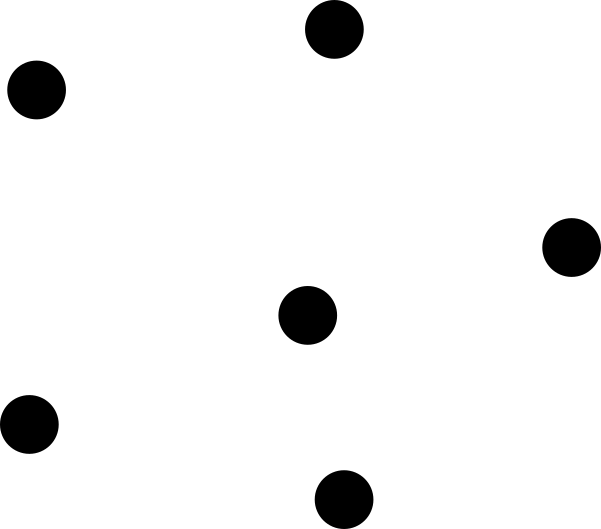
\includegraphics[width=.8\linewidth]{images/lab3/graph_sample_1.png}
    \caption{}
    \label{f:graph_sample_1}
  \end{subfigure}
  \begin{subfigure}{.25\textwidth}
    \centering
    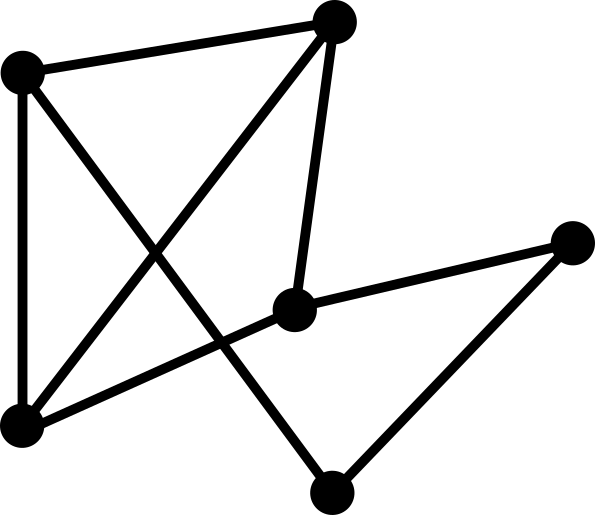
\includegraphics[width=.8\linewidth]{images/lab3/graph_sample_2.png}
    \caption{}
    \label{f:graph_sample_2}
  \end{subfigure}
  \begin{subfigure}{.25\textwidth}
    \centering
    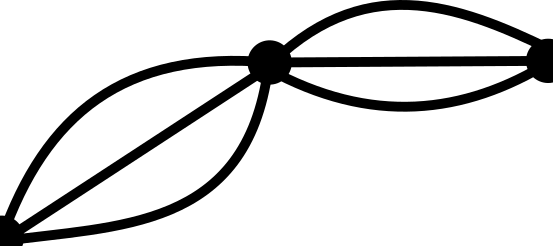
\includegraphics[width=.8\linewidth]{images/lab3/graph_sample_3.png}
    \caption{}
    \label{f:graph_sample_3}
  \end{subfigure}
  \begin{subfigure}{.25\textwidth}
    \centering
    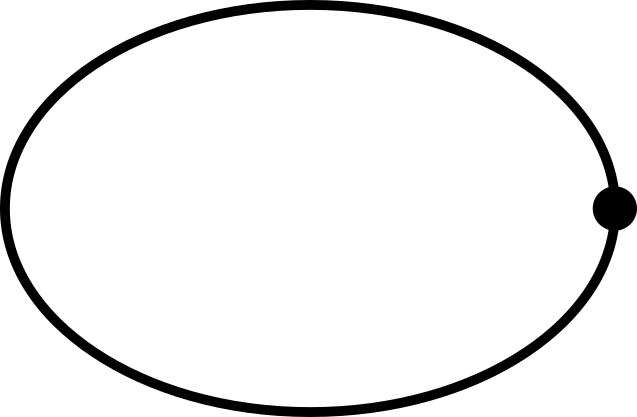
\includegraphics[width=.8\linewidth]{images/lab3/graph_sample_4.png}
    \caption{}
    \label{f:graph_sample_4}
  \end{subfigure}
  \begin{subfigure}{.25\textwidth}
    \centering
    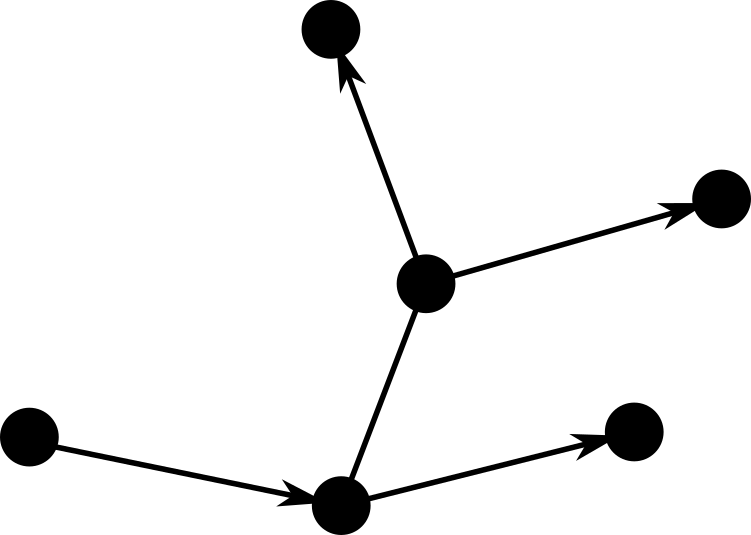
\includegraphics[width=.8\linewidth]{images/lab3/graph_sample_5.png}
    \caption{}
    \label{f:graph_sample_5}
  \end{subfigure}
  \begin{subfigure}{.25\textwidth}
    \centering
    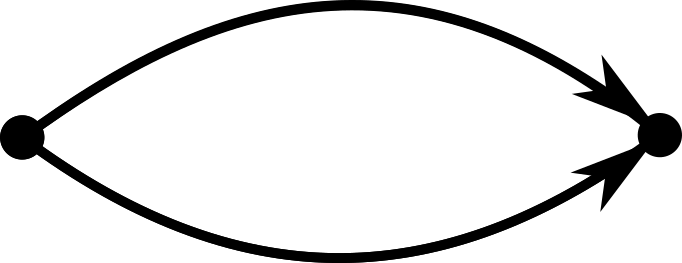
\includegraphics[width=.8\linewidth]{images/lab3/graph_sample_6.png}
    \caption{}
    \label{f:graph_sample_6}
  \end{subfigure}
  \begin{subfigure}{.25\textwidth}
    \centering
    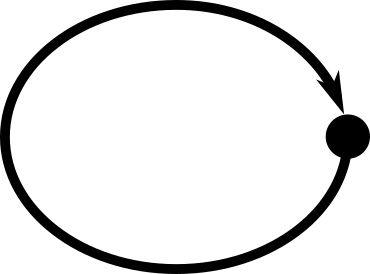
\includegraphics[width=.8\linewidth]{images/lab3/graph_sample_7.png}
    \caption{}
    \label{f:graph_sample_7}
  \end{subfigure}
  \begin{subfigure}{.25\textwidth}
    \centering
    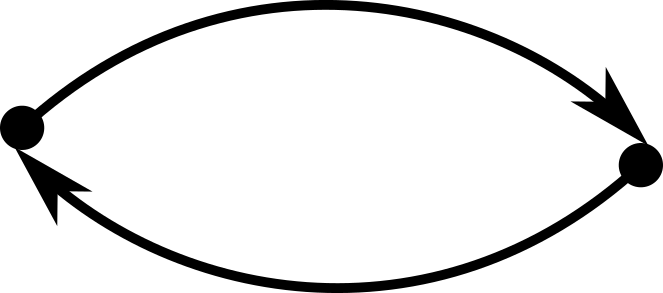
\includegraphics[width=.8\linewidth]{images/lab3/graph_sample_8.png}
    \caption{}
    \label{f:graph_sample_8}
  \end{subfigure}
  \caption{Приклади графічного представлення графів}
  \label{f:graph_examples}
\end{figure}


Якщо множина ребер $E$ порожня (\ref{f:graph_sample_1}), граф називається \emph{нуль-графом}. Якщо
множина вершин $V$ є порожньою, то порожньою є також множина ребер $E$. Такий граф називається
\emph{порожнім}.

Лінії, що зображають ребра графа, можуть перетинатися, але точки перетину не є
вершинами (\ref{f:graph_sample_2}).

Різні ребра можуть бути інцидентні одній і тій самій парі вершин (\ref{f:graph_sample_3}), такі ребра
називаються \emph{кратними} (випадок наявності однакових пар ($v_i$, $v_j$)). Граф, що містить
кратні ребра, називається \emph{мультиграфом}.

Ребро може з'єднувати вершину саму з собою (\ref{f:graph_sample_4}), таке ребро називається
\emph{петлею}. Це випадок наявності пар $(v_i, v_i)$. Граф із петлями та кратними ребрами
називається \emph{псевдографом}.

Якщо пара $e = (v, w) \in E$ вважається впорядкованою, тобто суттєвим є порядок розташування кінців
ребра (іншими словами, важливим є, яка вершина ребра є початком, а яка --- кінцем), то таке ребро
називається \emph{орієнтованим}. В такому випадку $(w, v) \neq (v, w)$. Граф, що містить лише
орієнтовані ребра, називається \emph{орієнтованим}.

Якщо немає різниці, яку вершину ребра вважати початком, а яку --- кінцем, тобто
$(w, v) = (v, w)$, ребро є \emph{неорієнтованим}. Граф, що містить тільки неорієнтовані
ребра --- \emph{неорієнтований}. Іноді граф може містити як орієнтовані, так і неорієнтовані ребра
(\emph{змішаний} граф). Ребра орієнтованого графа прийнято називати \emph{дугами} і позначати
направленими відрізками (\ref{f:graph_sample_5}). Напрямки орієнтованих ребер позначаються
стрілками. Орієнтований граф може мати кратні ребра (\ref{f:graph_sample_6}), петлі
(\ref{f:graph_sample_7}), а також петлі, що з'єднують одні й ті самі вершини, але у зворотних
напрямках (\ref{f:graph_sample_8}).

Кожному неорієнтованому графу можна поставити у відповідність орієнтований граф з тією самою
множиною вершин та множиною ребер, в якій кожне ребро замінено двома орієнтованими ребрами, що є
інцидентними тим самим вершинам та мають зворотні напрямки. Про дугу $(w, v)$ кажуть, що вона
виходить з вершини $w$ та приходить в вершину $v$.  Вершини $w$ та $v$ називають відповідно початком
та кінцем дуги $(w, v)$.

Задати граф означає задати множини його вершин та ребер, а також відношення інцидентності. Крім
графічного, є інші способи задання графа.  Якщо граф скінчений, для опису його вершин та ребер
достатньо їх занумерувати. Нехай $v_1, v_2 \ldots v_n$ --- вершини графа, $e_1, e_2, \ldots e_m$ --
його ребра. Відношення інцидентності можна визначити матрицею, що має $m$ рядків та $n$
стовпчиків і складається з елементів $\varepsilon_{ij}$. Стовбці відповідають вершинам
графа, а рядки -- його ребрам.

Якщо ребро $e_{i}$ є інцидентним вершині $v_{j}$, тоді елемент $\varepsilon_{ij} = 1$, інакше
$\varepsilon_{ij} = 0$.  Така матриця називається \emph{матрицею інцидентності} звичайного графа і є
одним зі способів його визначення. Для графа на \ref{f:sample_graph} --- матриця інцидентності
наведена в \ref{t:incidence_matrix}.

\begin{figure}[!ht]
  \centering
  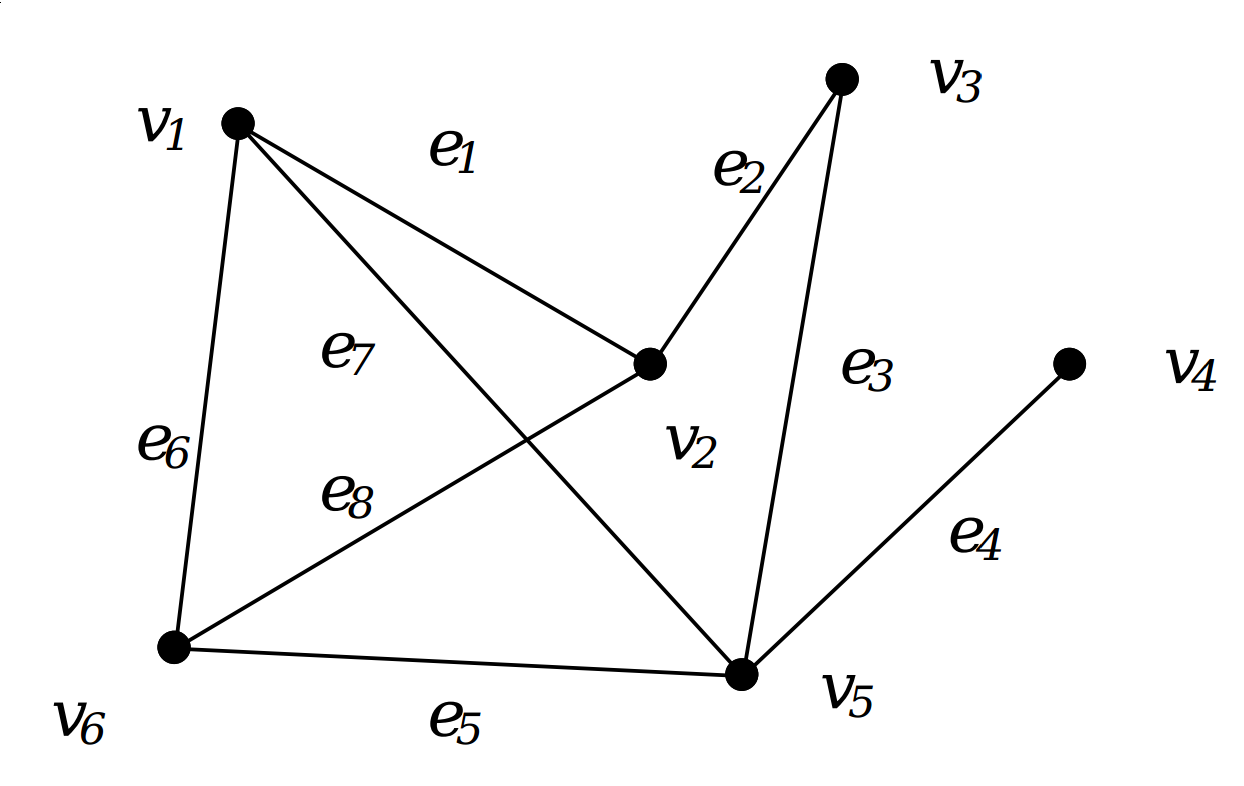
\includegraphics[width=.75\textwidth]{images/lab3/sample_graph.png}
  \caption{}
  \label{f:sample_graph}
\end{figure}

Для орієнтованого графа прийнято, що елемент $\varepsilon_{ij} = -1$, якщо вершина $v_{j}$ є
початком ребра $e_{i}$; $\varepsilon_{ij} = 1$, якщо вершина $v_j$ є кінцем ребра $e_{i}$;
$\varepsilon_{ij} = \alpha \not\in (-1, 0, 1)$, якщо $e_{i}$ --- петля інцидентної вершини $v_j$;
інакше $\varepsilon_{ij} = 0$.

Граф можна задати \emph{матрицею суміжності} --- квадратною матрицею $\delta_{ij}$, стовпцям і
рядкам якої відповідають вершини графа. Для неорієнтованого графа $\delta_{ij}$ дорівнює кількості
ребер, інцидентних $i$-тій та $j$-тій вершинам (кількості ребер, що їх з'єднують), для орієнтованого
графа цей елемент відповідає кількості ребер з початком в $i$-тій вершині та кінцем в $j$-тій
вершині. Таким чином матриця суміжності неорієнтованого графа є симетричною
$(\delta_{ij} = \delta_{ji})$, а орієнтованого --- необов'язково. Якщо ж вона є все-таки
симетричною, то для кожної дуги орієнтованого графа існує дуга, що з'єднує ті ж вершини, але в
зворотному напрямку.

Матриця суміжності для графа на \ref{f:sample_graph} наведена в таблиці \ref{t:adjacency_matrix}.

\begin{table}[!ht]
  \centering
  \caption{Матриця інцидентності}
  \label{t:incidence_matrix}
  \begin{tabular}{|c|c|c|c|c|c|c|c|}
\hline
& $v_1$ & $v_2$ & $v_3$ & $v_4$ & $v_5$ & $v_6$ \\ \hline
$e_1$ & 1 & 1 & 0 & 0 & 0 & 0 \\ \hline
$e_2$ & 0 & 1 & 1 & 0 & 0 & 0 \\ \hline
$e_3$ & 0 & 0 & 1 & 0 & 1 & 0 \\ \hline
$e_4$ & 0 & 0 & 0 & 1 & 1 & 0 \\ \hline
$e_5$ & 0 & 0 & 0 & 0 & 1 & 1 \\ \hline
$e_6$ & 1 & 0 & 0 & 0 & 0 & 1 \\ \hline
$e_7$ & 1 & 0 & 0 & 0 & 1 & 0 \\ \hline
$e_8$ & 0 & 1 & 0 & 0 & 0 & 1 \\ \hline
\end{tabular}                                                
\end{table}

\begin{table}[!ht]
  \centering
  \caption{Матриця суміжності}
  \label{t:adjacency_matrix}
  \begin{tabular}{|c|c|c|c|c|c|c|c|}
\hline
& $v_1$ & $v_2$ & $v_3$ & $v_4$ & $v_5$ & $v_6$ \\ \hline
$v_1$ & 0 & 1 & 0 & 0 & 1 & 1 \\ \hline
$v_2$ & 1 & 0 & 1 & 0 & 0 & 1 \\ \hline
$v_3$ & 0 & 1 & 0 & 0 & 1 & 0 \\ \hline
$v_4$ & 0 & 0 & 0 & 0 & 1 & 0 \\ \hline
$v_5$ & 0 & 0 & 1 & 1 & 0 & 1 \\ \hline
$v_6$ & 1 & 1 & 0 & 0 & 1 & 0 \\ \hline
\end{tabular}                                                
\end{table}

\emph{Маршрутом (шляхом) у графі} називається така скінченна або нескінченна послідовність вершин і
ребер, що чергуються:

$$(\ldots \emph{v_{1}, e_{1}, v_{2,} e_{2}, \ldots, v_{n-1}, e_{n-1}, v_{n},} \ldots)$$,

що кожні два сусідні ребра $e_{i-1}$ та $e_{i}$ мають спільну інцидентну вершину $v_{i}$. В
скінченних маршрутах існує перше та останнє ребра, а також перша (початок маршруту) та остання
(кінець маршруту) вершини.

Граф називається \emph{зваженим}, якщо на множині ребер визначено вагову функцію (кожному ребру
поставлена у відповідність вага). Для будь-якого шляху $М$ зваженого графу позначимо через $l(M)$
суму ваг ребер, що входять у $М$. Величину $l(M)$ будемо називати \emph{вагою (або довжиною)} шляху
$М$ у зваженому графі. Шлях у зваженому графі з вершини $w$ в вершину $v$, де $w≠~v$,
називається \emph{мінімальним}, якщо він має найменшу вагу серед усіх шляхів з вершини $w$ в
вершину $v$.

Існує багато практичних задач, що зводяться до пошуку мінімального шляху на графах (задачі
мінімізації транспортних, енергетичних, інформаційних тощо потоків, пошуку оптимальних
послідовностей виконуваних дій, наприклад оптимальної послідовності запуску партій виробів тощо).

Розглянемо \textbf{\emph{алгоритм знаходження}} оптимального за мінімумом довжини (найкоротшого)
\textbf{\emph{шляху}} в неорієнтованому графі з ребрами довільної довжини (ваги). Нехай задано граф,
у якого відомо ваги всіх ребер та вершини якого пронумеровано за порядком. Також задано початкову та
кінцеву вершини шляху (яка точка є початком, а яка є кінцем, значення не має). Позначимо початок
шляху -- $А$, кінець -- $В$. Нехай вага ребра, що з'єднує $i$-ту та $j$-ту вершини, буде позначатися
$L_{ij}$. Алгоритм передбачає присвоєння кожній вершині певного індексу (аналог потенціалу в
електричних схемах) та має два етапи -- етап визначення індексів всіх вершин та етап прокладання
шляху по ребрам, вага яких рівна різниці індексів інцидентних вершин (вершин, які з'єднуються даним
ребром).  Отже,

\begin{enumerate}

\item Визначення індексів вершин (позначатимемо $\lamda_{i}$ індекс вершини $v_{i}$).
\item  1.1. Приймаємо індекс вершини кінця шляху (\emph{В}), рівний 0:
$\lambda_{(B)} = 0$.

1.2. Починаємо цикл по всім вершинам, починаючи з вершини \emph{В}. Для
кожної вершини, індекс якої відомий, виконуємо визначення індексів всіх
суміжних вершин. Якщо індекси всіх суміжних вершин для даної буде
визначено, то така вершина буде вважатися ``пройденою'' і біля неї
поставимо галочку.

1.2.1. Починаємо цикл індексації по всім вершинам, сусіднім з даною. Для
кожної сусідньої вершини виконуємо:

1.2.1.1. Визначення можливого індексу чергової вершини:
\lambda_{j} = \lambda\emph{_{i}} +
\emph{L_{ij}} (\lambda\emph{_{i}} -- індекс вершини,
відносно якої визначаємо);

1.2.1.2. Якщо індекс даної вершини, яку розраховуємо, ще не був
визначений або є більший, ніж нове розраховане значення
\lambda_{j}, приймаємо його рівним новому значенню
\lambda_{j}, інакше -- не змінюємо.

1.2.2. Повторюємо пп.1.2.1.1--1.2.1.2 для всіх вершин, сусідніх з даною.
Після цього дану вершину вважаємо ``пройденою'' і біля неї поставимо
галочку. Якщо при розрахунку індексів сусідніх вершин змінився індекс
вершини, яка буда ``пройденою'', вона перестає бути ``пройденою'' і
галочка біля неї знімається.

1.2.3. Повторюємо п.1.2.1--1.2.2 доки всі вершини (крім \emph{А}) не
будуть ``пройдені'' (біля них будуть стояти галочки). Довжина шляху
рівна індексу вершини \emph{А}.

2. Визначення шляху.

2.1. Починаючи з вершини, що є початком шляху (\emph{А}), визначаємо
чергове ребро, по якому іде шлях. Це буде ребро, що з'єднує дану вершину
\emph{v_{j}} з вершиною \emph{v_{i}}, різниця
індексів яких в точності рівна вазі ребра: \lambda_{j} --
\lambda\emph{_{i}} = \emph{L_{ij}}
(\lambda_{j} -- останньої знайденої вершини,
\lambda\emph{_{i}} -- індекс вершини, що перевіряється на предмет
того, щоб вона стала наступною в мінімальному шляху). Завжди знайдеться
принаймні одне таке ребро, що з'єднує дану вершину з вершиною, відносно
якої був порахований індекс даної.

2.2. Повторюємо п.2.1., поки не прийдемо в вершину \emph{В}. Якщо на
якомусь кроці пункту 2.1 задовольняє декілька ребер, маємо альтернативні
шляхи і виконуємо далі п.2.1 для кожного із шляхів.

Цікавою представляється задача синтезу графа -- побудови такого графа, в
якому оптимальний шлях має бути таким, як заздалегідь визначено
(наприклад, якщо треба спроектувати транспортну або інформаційну мережу
так, щоб в ній певний потік проходив саме так, як визначено). Розглянемо
\textbf{\emph{алгоритм побудови (синтезу) графа}} (визначення ваги всіх
ребер та індексів всіх вершин), що має задану структуру, заданий
оптимальний шлях та якомога меншу сумарну вагу всіх ребер. Структура
графу (набір вершин та ребер, що їх з'єднує), береться як у графа в
задачі визначення оптимального шляху. Заданий шлях отримується
дзеркальним відображенням знайденого шляху відносно горизонтальної
прямої. Довжина шляху береться більшою (меншою) довжини знайденого шляху
на константу, вказану викладачем. Алгоритм полягає в наступному:

1. Малюємо дзеркальний граф, на якому позначаємо заданий шлях.
Розподіляємо загальну довжину заданого шляху по ребрам, що його
складають (приблизно рівномірно).

2. Приймаємо індекс кінця шляху (\emph{В}), рівний 0:
\lambda_{(B)} = 0.

3. Визначаємо індекси вершин, по яким проходить оптимальний шлях:
\lambda_{j} = \lambda\emph{_{i}} +
\emph{L_{ij}} (поки не дійдемо до вершини \emph{А}).

4. Визначаємо ваги інших ребер та індекси вершин (що не належать
оптимальному шляху):

4.1.Для ребра, що має визначені індекси обох кінців:

4.1.1. Якщо вершина, якій відповідає більший індекс, належить
оптимальному шляху -- вага ребра рівна різниці індексів вершин плюс 1.
Інакше -- вага ребра рівна різниці індексів вершин (але не менша 1):
L_{ij} = \lambda_{j} -- \lambda\emph{_{i}+1},
якщо \lambda_{j} \textgreater{} \lambda\emph{_{i}} та
\lambda_{j} \emph{∈ (AB)_{min}}, інакше:
L_{ij} = max((\lambda_{j} --
\lambda\emph{_{i}}), 1).

4.2. Для вершини, індекс якої невідомий, визначаємо сусідню з
мінімальним індексом. Індекс даної вершини буде на 1 більше індексу
сусідньої вершини з мінімальним індексом.

4.3. Виконуємо 4.1-4.2 поки всі індекси вершин та ваги ребер не будуть
визначені.
